\section{Introduction}

In this chapter, we present an efficient defect control technique for use in the numerical solution of initial value ordinary differential equations (ODE). We will assume that the underlying numerical method is a Runge-Kutta (RK) method since the vast majority of the literature on the use of defect control for numerical solution of IVODEs focuses on RK methods. Solvers based on Runge-Kutta methods only provide a discrete numerical solution. They adaptively divide the time domain into steps and return an estimate of the solution at the end of each step. To get a continuous solution approximate, the user has to fit an interpolant over the whole region.

The issue is that there is no guarantee that the interpolant will be as accurate as the discrete solution calculated by the solver. Thus if the solver returned a solution that satisfied a tolerance of $10^{-i}$, there are no guarantee that in the middle of a step, the interpolant will also deliver approximate solution values whose accuracy is approximately $10^{-i}$. 

High quality contemporary IVODE solvers typically have a built-in interpolant that provides a continuous solution approximation. However the solvers typically do not provide any type of explicit control of the accuracy of the continuous solution approximate. We show in Section $\ref{section:end_of_step_innacurate}$, that even for the robust IVODE solvers in Python, using interpolation does not guarantee solution approximations that have the same accuracy as the solution approximations at the end of each step. 


There has been some work towards addressing this issue in the area of control of the defect of the continuous solution approximation \cites{MR2600928}{MR1950917}{MR1803189}{MR1239829}{MR997658}{MR996053}. The defect is the amount by which the continuous solution approximation fails to satisfy the IVODE. We discuss this work in Section $\ref{section:crk_related_work}$. Typically, the interpolants employed in algorithms for defect control are based on the use of Continuous Runge-Kutta methods and the computational costs are substantial. 

In this paper we will discuss an efficient method for defect control of the continuous solution using multistep Hermite Birkhoff interpolants. For related work, see \cites{MR1239829}{tsitouras1990runge}{papageorgiou1997continuous} and the references within. We will control an estimate of the maximum defect along a step and show how that yields a continuous solution approximation over the whole time domain whose defect is typically within the tolerance.

We start by discussing the ODE problems we will use to demonstrate our approach in Section $\ref{section:defect_problem_used}$. We then give an overview of the issue with using error control only at the end of the step in Section $\ref{section:end_of_step_innacurate}$. We discuss related work in Section $\ref{section:crk_related_work}$. We give a description of the solvers that we use in Section $\ref{section:basic_runge_kutta}$. 

We discuss several multistep interpolants that we have constructed based on a Runge-Kutta method of order 4 in Section $\ref{section:equipping_rk4_with_HBs}$ and extend them to higher order Runge-Kutta methods in Section $\ref{section:HBs_and_higher_order_RK}$. We then discuss possible solutions to a fundamental issue with our approach in Section $\ref{section:keeping_alpha_at_1}$ and give some final recommendations on building a final solver in Section $\ref{section:defect_final_recommendations}$.

\subsection{Test Problems}
\label{section:defect_problem_used}
In this section, we discuss the three problems that we use \cite{MR1421071}. 

The first problem has the ODE:
\begin{equation}
y'(t) = - \frac{y^{3}(t)}{2} 
\end{equation}
The initial condition is $y(0) = 1$ and the time domain is $[0, 10]$.

The solution to this problem is
\begin{equation}
y(t) = \frac{1}{\sqrt{1 + t}}.
\end{equation}
as shown in Figure $\ref{fig:solution_problem1}$.

\begin{figure}[H]
\centering
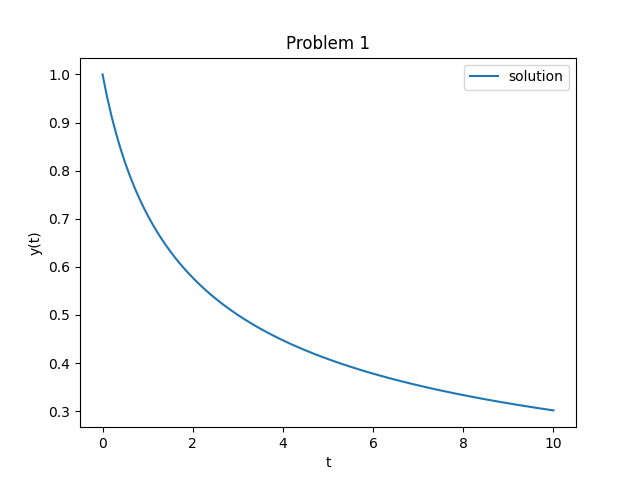
\includegraphics[width=0.7\linewidth]{./figures/solution_problem1}
\caption{Solution to the first ODE problem.}
\label{fig:solution_problem1}
\end{figure}

The second problem has the ODE:
\begin{equation}
y'(t) = \frac{y(t)(1 - \frac{y(t)}{20})}{4}.
\end{equation}
The initial condition is $y(0) = 1$ and the time domain is $[0, 10]$.

The solution to this problem is
\begin{equation}
y(t) = \frac{20e^{\frac{t}{4}}}{e^{\frac{t}{4}} + 19},
\end{equation}
as shown in Figure $\ref{fig:solution_problem2}$.

\begin{figure}[H]
\centering
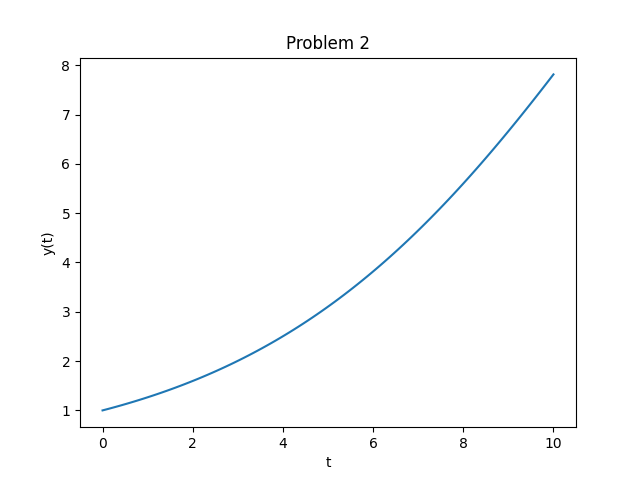
\includegraphics[width=0.7\linewidth]{./figures/solution_problem2}
\caption{Solution to the second ODE problem.}
\label{fig:solution_problem2}
\end{figure}

The third problem has the ODE:
\begin{equation}
y'(t, y) = -0.1y - e^{-0.1t}\sin(t)
\end{equation}
The initial condition is $y(0) = 1$ and the time domain is $[0, 10]$.

The solution to this problem is 
\begin{equation}
y(t) = e^{-0.1t}\cos(t),
\end{equation}
as shown in Figure $\ref{fig:solution_problem3}$.

\begin{figure}[H]
\centering
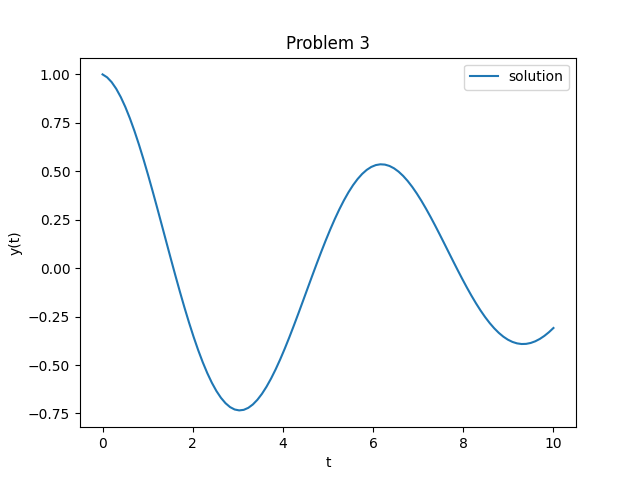
\includegraphics[width=0.7\linewidth]{./figures/solution_problem3}
\caption{Solution to the third ODE problem.}
\label{fig:solution_problem3}
\end{figure}

\subsection{Absence of control of the continuous solution approximation for typical IVODE solvers}
\label{section:end_of_step_innacurate}
In this section, we discuss how conventional solvers employed in popular packages like the Scipy library solve IVODE problems. These libraries will often have the option of using an error control solver based on a Runge-Kutta pair which works as follows. The pair comes with a low order method and a high order method and will solve an ODE by taking a sequence of steps. The solver will take each step with both methods and use the difference between the higher order method and the lower order method to generate an error estimate for the discrete numerical solution at the end of the step. If the error estimate is within the user provided tolerance, the solver will accept the step and proceed to the next step. If the error estimate is not within the tolerance, the solver will reduce the step-size and attempt to take the step again. As the error of Runge-Kutta methods depends on the step-size, a smaller step-size will produce a smaller error. The solver will keep reducing the step-size until the user tolerance is satisfied and will then proceed to the next step. In an attempt to improve the efficiency, solvers will also increase the step-size when the estimated error is significantly smaller than the tolerance.

An issue with this approach is that the error estimate is computed only for the discrete numerical solution computed at the end of a step and thus the error control is only applied at the end of the step. An interpolant that provides a continuous solution approximation across the entire step is typically constructed by the solver and it is hoped that the error of the interpolant at points within the step is within the user-provided tolerance. However, as we will show below, this is sometimes not the case.

For this interpolant to provide a solution within the user provided tolerance, the theoritical interpolation error must be less than or equal to the error of the data being fitted. Thus we would ideally use an interpolant of at least order $O(h^{p})$ if the discrete solution is of order $O(h^{p})$. However, for high order methods, it becomes too expensive to construct an interpolant of the appropriate order. IVODE solvers will thus usually compromise and employ a lower order interpolant, that is less costly, but deliver less accuracy. 

Therefore, we are not guaranteed that the continuous approximate solution is error-controlled and not guaranteed that the interpolation error will not affect the continuous solution approximation. Figures $\ref{fig:no_middle_step_error_control_p2_dop853}$ and $\ref{fig:no_middle_step_error_control_p3_rk45}$ show some results obtained when Runge-Kutta solvers are applied to some of the test problems introduced in the previous section. In these figures, we plot the global error of the numerical solution, this is the difference between the exact solution and the computed solution over the time domain. The solvers apply error control to the discrete numerical solution at the end of the step but no error control of any type to the continuous numerical solution across the step.

\begin{figure}[H]
\centering
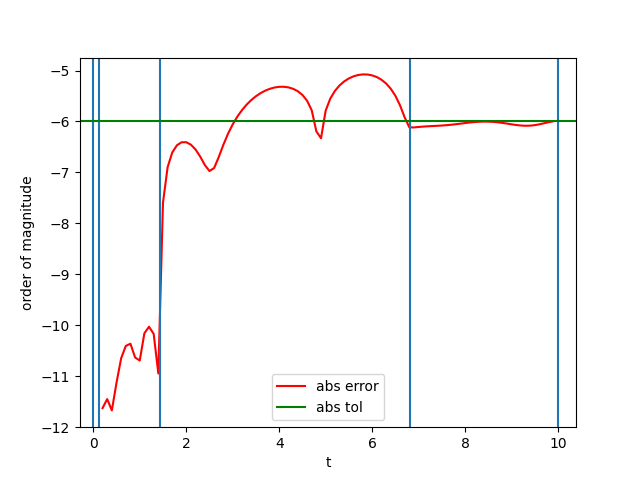
\includegraphics[width=0.7\linewidth]{./figures/no_middle_step_error_control_p2_dop853}
\caption{The Python `DOP853' solver on problem 2 with an absolute tolerance of $10^{-6}$ and a relative tolerance of $10^{-6}$. Steps are represented by the vertical lines.}
\label{fig:no_middle_step_error_control_p2_dop853}
\end{figure}

\begin{figure}[H]
\centering
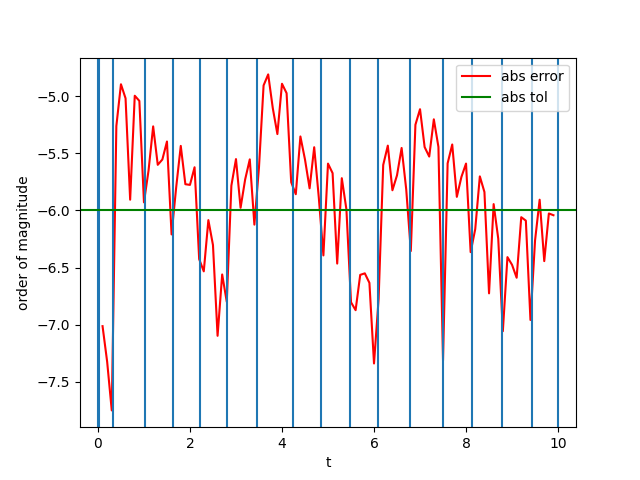
\includegraphics[width=0.7\linewidth]{./figures/no_middle_step_error_control_p3_rk45}
\caption{The Python `RK45' solver on problem 3 with an absolute tolerance of $10^{-6}$ and a relative tolerance of $10^{-6}$. Steps are represented by the vertical lines.}
\label{fig:no_middle_step_error_control_p3_rk45}
\end{figure}

Figure $\ref{fig:no_middle_step_error_control_p2_dop853}$ and $\ref{fig:no_middle_step_error_control_p3_rk45}$ shows the errors in the middle of each step obtained when applying `DOP853' to problem 2 and `RK45' to problem 3 with an absolute tolerance of $10^{-6}$ and a relative tolerance of $10^{-6}$. We can see that the solution values at the end of each step typically satisfy the tolerance. However we can clearly see that the solution values (obtained from the built-in interpolant constructed by the solver) at points within each steps, have errors up to one order of magnitude larger than the tolerance. 

We note that when a user asks for a solution whose estimated error is within a tolerance of $10^{-i}$, they expect the solution to have an estimated error that is within that tolerance for the whole time domain. However, the decision to not satisfy the user provided tolerance throughout the step is made in the interest of efficiency and the loss of accuracy in the middle of the step is the tradeoff. The goal of modern IVODE solvers is to provide a continuous solution approximation across the whole time domain. The user's expectation is that the solution approximations across each step also satisfies the tolerance as ODE solvers can be integral part of larger software packages where their approximate solutions are differentiated, integrated and manipulated in ways such that a sufficiently accurate continuous approximate solution is required. 

In this chapter, we attempt to provide an efficient way of constructing interpolants that can then be used to control the defect of the continuous approximate solution across the step and thus throughout the whole time domain.

\subsection{Defect control and the cost of traditional Continuous Runge-Kutta methods}
\label{section:crk_related_work}
In this section we introduce the `defect' of a continuous approximate solution of an ODE and explain how the control of that defect provides a type of error control of the continuous numerical solution.

In the context of numerical ODEs, the defect, denoted by $\delta(t)$,  is the amount by which the continuous numerical solution, $u(t)$, fails to satisfy the ODE. When the ODE is $y'(t) = f(t, y(t))$, the defect is 

\begin{equation}
\delta(t) = |u'(t) - f(t, u(t))|.
\end{equation}

Calculating the defect requires that the continuous approximate solution computed by the solver to also be differentiable. The idea of defect control is relatively new as differentiable solutions to ODEs can be expensive to calculate. Several investigations in this direction are outlined in \cites{MR2600928}{MR1950917}{MR1803189}{MR1239829}{MR997658}{MR996053}. In this work, the defect control method employs a continuous RK method for which the number of stages grows exponentially with the order of the method as shown in Table $\ref{tab:crk_nstages}$. In this chapter, we will compute a defect controlled continuous solution with no additional cost. A typical Runge-Kutta solver will thus be able to employ the usual number of stages required for the discrete Runge-Kutta method and still produce an accurate continuous solution.

\begin{table}[h]
\caption {Number of stages for discrete vs continuous RK method.} 
\label{tab:crk_nstages}
\begin{center}
\begin{tabular}{ c c c c} 
order   & discrete & continuous & asymptotically correct defect \\ 
4 & 4  & 4   & 8 \\ 
5 & 5  & 6   & 12 \\ 
6 & 6  & 7   & 15 \\ 
7 & 7  & 9   & 20 \\ 
8 & 8  & 13  & 27 \\ 
\end{tabular}
\end{center}
\end{table}

Though the defect is defined for the whole step, the estimation of the maximum defect within a step is what is important. If the maximum defect is within the tolerance, then the defect of the whole solution within the given step is within the tolerance. The key task is to find the location of the maximum defect within the step. One approach would be to sample the defect at several points and use the maximum value sampled. The problem with this approach is that each sampling of the defect requires an additional function evaluation. Thus we should not do too many samples. Work in this direction (cited above) involves constructing special interpolants that guarantee that (asymptotically) the maximum defect is at the same location within every step for every problem. This way only one function evaluation is required to sample the defect to obtain an estimate of the maximum defect. This is referred to as asymptotically correct defect control.

In the approach outlined in this chapter, we have observed experimentally that the maximum defect will tend to appear at one of two locations within the step. Thus in our approach, only two defect samplings must be done to get the maximum defect. Though we make an additional function evaluation compared to the asymptotically correct defect control, using no function evaluations to construct the interpolant guarantees that our method is more efficient especially for higher orders.

============================================================
I dont think we can put the Butcher Tablau, the numbers are too big.
I think we can just reference Jim Verner's website for crk65 and crk87.
Rk4 is the classical rk4 currently. You might want to gievv me a crk4 but we ruled that out as it does seem that crk4 will be much better than rk4 with hb6 as it makes only one additional stage.

I included the following rk6 and rk8:
the rk6 is his 'most efficient pair': https://www.sfu.ca/~jverner/RKV65.IIIXb.Efficient.00000144617.081204.RATOnWeb for which he gave a 5th and 6th order interpolant at a cost of +1 and +2 more function evaluations.

the rk8 is his 'most efficient pair' again: https://www.sfu.ca/~jverner/RKV87.IIa.Efficient.000000282866.081208.FLOAT40OnWeb for which he gave a 7th and 8th order interpolant at a cost of +4 and +4 additional function evaluations
============================================================

\subsection{Overview of our approach}
\label{section:basic_runge_kutta}
In this chapter, we will discuss simple IVODE solvers based on discrete Runge-Kutta methods of order 4, 6 and 8 and show that we can provide accurate continuous interpolant to augment the discrete solution computed by these RK methods without having to compute any additional function evaluations. In this section, we give an outline of the approach.

The first Runge-Kutta method upon which we build a prototype defect control solver is the classical $4^{th}$ order method that uses 4 stages; the second method is a Verner $6^{th}$ order method, taken from his 6(5) pair \cite{JimVernerRepo} that uses 9 stages, and the last method is a Verner $8^{th}$ order method from an 8(7) pair that uses 13 stages \cite{MR1239829}. 

The solvers that we have written use a simple step selection strategy. If the estimated maximum defect is greater than $tol$, the solver rejects the step and attempts to retake it again with half the step-size. If the estimated maximum defect is less than $0.1tol$, the solver accepts the step and doubles the step-size for the next step. We will elaborate on the initial step-size used by each solver later in the chapter.

We now note that the solver is not optimised. A more thorough analysis of how the solver behaves and thus a more refined step selection algorithm will produce a better solver in practice. The software we consider in this chapter only serves as a proof of concept for a more elaborate solver. 